\documentclass[a4paper, 12pt, final, garamond]{book}
\usepackage{cours-preambule}

\raggedbottom

\makeatletter
\renewcommand{\@chapapp}{M\'ecanique -- chapitre}
\makeatother

\begin{document}
\setcounter{chapter}{4}

\chapter{Correction TD entra\^inement}

\section{Séparation isotopique}
\begin{enumerate}
    \item Les ions étant positifs, ils subissent la force $\Ff_e = q\Ef$ dans le
        même sens que $\Ef$. Il faut donc que $\Ef$ soit selon $\uy$. Or, $\Ef =
        -\gd V$ indique que $\Ef$ va des hauts potentiels aux bas potentiels
        ($\gd$ indique le sens des grandes variations, $-\gd$ indique
        l'inverse)~: on veut donc que $V_P$ soit plus grand que $V_{P'}$, soit
        \[U_{PP'} = V_P - V_{P'} > 0\]

    \item L'ion, assimilable à un point matériel M$_i$, de masse $m_i$, est
        soumis dans le référentiel du laboratoire supposé galiléen à la force
        électrique qui est conservative. Donc le système est conservatif~:
        $\Ec_m(P)=\Ec_m(P')$. L'énergie potentielle électrique s'écrit
        $\Ec_p=qV$ (on prend la constante nulle), on part à vitesse nulle et on
        accélère jusqu'à $P'$, d'où

        \[
            qV(P)=\frac{1}{2}m_iv_i{}^2+qV(P')
            \quad\Ra\quad
            \boxed{v_i=\sqrt{\frac{2qU_{PP'}}{m_i}}} 
        \]
    \item
        Cf.\ cours~: $R_i=\frac{mv_i}{\abs{q}B}$, donc
        $R_i=\frac{\sqrt{2Um_i}}{B\sqrt{q}}$
        \begin{itemize}[label=$\diamond$, leftmargin=10pt]
            \litem{BDF~:}
                \[
                    \begin{array}{ll}
                        \textbf{Poids} & \text{négligeable \textbf{devant }}\Ff\\
                        \textbf{Force magnétique} & \Ff = q\vf\wedge\Bf =
                            \mqty(q\xp\\q\yp\\q\zp)\wedge\mqty(0\\0\\B)\\
                                            \Lra & \Ff = q\yp B\ux -q\xp B\uy 
                    \end{array}
                \]
            \litem{PFD~:}
                \[m_i\af = \Ff\]
            \litem{Équations scalaires~:}
                \begin{empheq}[left=\empheqlbrace]{align*}
                    m_i\xpp &= q\yp(t)B\\
                    m_i\ypp &= -q\xp(t)B\\
                    m_i\zpp &= 0
                \end{empheq}
        \end{itemize}
        D'où~:
        \begin{gather*}
            \left\{
                \begin{aligned}
                    \xpp(t) &= \frac{qB}{m_i}\yp(t)\\
                    \ypp(t) &= -\frac{qB}{m_i}\xp(t)
                \end{aligned}
            \right.
            \Lra
            \left\{
                \begin{aligned}
                    \xp(t) &= \frac{qB}{m_i}y(t) + K\\
                    \yp(t) &= -\frac{qB}{m_i}x(t) + K'
                \end{aligned}
            \right.
        \end{gather*}
        ainsi avec les conditions initiales~:
        \begin{gather*}
            \xp(0) = 0
            \qor
            \xp(0) = \frac{qB}{m_i}\underbracket[1pt]{y(0)}_{=0} + K = K
            \qdonc
            K = 0\\
            \yp(0) = v_i
            \qor
            \yp(0) = -\frac{qB}{m_i}\underbracket[1pt]{x(0)}_{=0} + K' = K'
            \qdonc
            K' = v_i
        \end{gather*}
        Soit
        \begin{empheq}[left=\empheqlbrace]{align*}
            \xp(t) &= \frac{qB}{m_i}y(t)\\
            \yp(t) &= -\frac{qB}{m_i}x(t) + v_i
        \end{empheq}
        Étant donné que $v_x(t)^2 + v_y(t)^2 = \cte = v_0{}^2$, on a
        \[\left(\frac{qB}{m_i}y(t)\right)^2 + \left(-\frac{qB}{m_i}x(t) + v_i\right)^2 =
        v_i{}^2\]
        soit, en notant $\w_c = \abs{q}B/m_i$~:
        \[\left(y\right)^2 + \left(x + \frac{m_iv_i}{qB}\right)^2 =
            \left( \frac{v_i}{\w_c} \right)^2\]
        On reconnaît l'équation d'un cercle en coordonnées cartésiennes. Dans
        notre cas, les centres sont $\DS\left(-\frac{m_iv_i}{qB},0\right)$ et les
        rayons sont $\DS R_i = \frac{v_i}{\w_c} = \frac{m_iv_i}{\abs{q}B}$, soit
        \[\boxed{R_i = \frac{\sqrt{2Um_i}}{B\sqrt{q}}}\]
    \item Graphiquement, on a $d=2(R_2-R_1)$. Donc
	\[
        \boxed{d=\cfrac{2\sqrt{2}}{B}
        \sqrt{\cfrac{U}{q}}\left(\sqrt{m_2}-\sqrt{m_1}\right)}
    \]
\end{enumerate}

\section{Cyclotron}
\begin{itemize}[label=$\diamond$]
    \litem{Système}~: {proton}, assimilé à un point matériel de masse $m$ et de
        charge $q$.
    \litem{Référentiel}~: lié au cyclotron, donc référentiel du laboratoire
        supposé galiléen.
    \litem{BDF}~:
        \[
            \begin{array}{ll}
                \textbf{Poids} & \text{négligeable \textbf{devant }}\Ff\\
                \textbf{Force de \textsc{Lorentz}} & \Ff = e(\Ef + \vf\wedge\Bf)
            \end{array}
        \]
\end{itemize}
\begin{enumerate}
    \item À l'intérieur des \textit{dees}, seule la force magnétique $\Ff_m =
        e\vf\wedge\Bf$ existe. Ainsi, d'après le TEM,
        \[
            \dv{\Ec_c}{t} =
            e\underbracket[1pt]
            {\underbracket[1pt]
            {\vf\wedge\Bf}_{\perp\vf}\cdot\vf}_{=0} = 0
            \qsoit
            mv\dv{v}{t} = 0
            \qMath{d'où}
            \boxed{\dv{v}{t} = 0}
        \]
    \item La trajectoire d'un proton dans un champ magnétique est un arc de
        cercle, parcouru à vitesse constante. Utilisons un repérage
        \textbf{polaire}, centré sur le centre de l'arc de cercle. D'après la
        deuxième loi de \textsc{Newton},
        \[m\af = e\vf\wedge\Bf\]
        soit en utilisant les résultats connus sur la cinématique du mouvement
        circulaire,
        \[m\left(-\frac{v^2}{R}\ur\right) =
        evB\underbracket[1pt]{(-\ut\wedge\uz)}_{=\ur} = -evB\er\]
        avec $\vf = -v\ut$~: la trajectoire est parcourue en sens horaire pour
        un proton (à connaître ou à retrouver par la cohérence des signes).
        Finalement,
        \[
            \frac{mv^2}{R} = evB
            \qMath{d'où}
            \boxed{R = \frac{mv}{eB}}
        \]
        La trajectoire dans un des \textit{dee} est ainsi un demi-cercle, de
        longueur $\pi R$ et, \textbf{puisque la vitesse est constante},
        parcourue en un temps
        \[
            \boxed{\D t_d = \frac{\pi R}{v} = \frac{\pi m}{eB} = \SI{22}{ns}}
        \]
        On remarque ainsi que $\D t_d$ ne dépend pas de la vitesse du proton,
        mais seulement du champ appliqué dans le \textit{dee} (en plus des
        variables intrinsèques au proton, $e$ et $m$).
    \item Pour que le proton soit accéléré de façon optimale à chaque passage
        entre les \textit{dees}, il faut que la force électrique qu'il subit
        soit alternativement orientée selon $+\ux$ lorsqu'il passe de $D_2$ à
        $D_1$, et selon $-\ux$ en passant de $D_1$ à $D_2$. En négligeant le
        temps de passage dans l'espace entre les \textit{dees} ($a \ll \pi R$),
        il faut donc qu'une demi-période de la tension appliquée soit égale à
        $\D t_d$, soit pour une période entière~:
        \[
            T = 2\D t_d = \frac{2\pi m}{eB}
            \qet
            \boxed{f = \frac{eB}{2\pi m} = \SI{23}{MHz}}
        \]
        Utiliser une tension harmonique plutôt qu'une tension créneau a
        l'intérêt de regrouper tous les protons pour que leur passage dans les
        \textit{dees} soit en phase avec la tension. Regrouper les protons
        permet aux impulsions du faisceau d'être plus puissantes. De plus, en
        pratique, un tension créneau requiert beaucoup d'harmoniques qu'il peut
        ne pas être simple d'imposer à de telles fréquences.

    \item Jusqu'à présent, nous avons relié le rayon à la vitesse du proton. Il
        faut donc maintenant relier la vitesse du proton au nombre de passage
        dans les \textit{dees}, ou plutôt au nombre de passage dans la zone
        accélératrice. Comme on ne s’intéresse qu'à la norme, le théorème de
        l'énergie cinétique est le plus adapté. Appliquons ce théorème sur une
        trajectoire entre la sortie d’un \textit{dee} et l'entrée de l'autre, en
        supposant que le passage du proton se fait au moment où la tension
        atteint son maximum (justifié par la question précédente), et en
        supposant aussi que la durée de passage dans la zone accélératrice est
        négligeable devant la période de la tension, ce qui permet de supposer
        que la tension est presque constante égale à $U_m$. Sous ces hypothèses,
        on trouve~:
        \[
            \frac{1}{2}mv_{n+1}{}^2 - \frac{1}{2}mv_n{}^2 = W(\Ff_e) =
            e\frac{U_m}{a}a
        \]
        En raisonnant par récurrence, on obtient
        \[
            \frac{1}{2}m v_n{}^2 - \frac{1}{2}mv_0{}^2
            \approx \frac{1}{2}mv_n{}^2 = neU_m
            \qsoit
            v_n = \sqrt{\frac{2neU_m}{m}}
        \]
        et en utilisant le résultat d'une question précédente,
        \[
            R_n = \frac{m}{eB} \sqrt{\frac{2neU_m}{m}}
            \qsoit
            \boxed{R_n = \sqrt{\frac{2nmU_m}{B^2e}}}
        \]
    \item Remarquons bien que $n$ compte le nombre de passages dans la zone
        accélératrice, faire un tour complet revient donc à passer de $n$ à
        $n+2$. Après un seul tour, $n=2$, et
        \[
            v_2 = \sqrt{\frac{4eU_m}{m}}
            \qet
            R_2 = 2 \sqrt{\frac{mU_m}{eB^2}} = \SI{6.1}{cm}
        \]
        Après dix tours, $n = 20$ et
        \[
            \boxed{R_{20} = \sqrt{10}R_2 = \SI{19}{cm}}
        \]
    \item Avec $R_N = \SI{35}{cm}$, la vitesse finale vaut
        \[
            v_{\rm fin} = \frac{eBR_N}{m}
            \qMath{d'où}
            \boxed{\Ec_{c,\rm fin} = \frac{e^2B^2R_N{}^2}{2m}
                = \SI{2.1e-12}{J} = \SI{14}{MeV}}
        \]
        puis
        \[
            \Ec_{c,\rm fin} = NeU_m
            \qMath{d'où}
            \boxed{N = \frac{\Ec_{c,\rm fin}}{eU_m} = 33}
        \]
        ce qui correspond à 16 tours et demi au sein du cyclotron.
\end{enumerate}

\section{Chambre à bulles}
\begin{enumerate}
    \item Dans le référentiel terrestre supposé galiléen, la particule P n'est
        soumise qu'à la force magnétique $\Ff = q\vf\wedge\Bf$, en négligeant le
        poids devant cette force. Avec le principe fondamental de la dynamique,
        on trouve
        \begin{gather*}
            \left\{
                \begin{aligned}
                    m\xpp &= q\yp(t)B\\
                    m\ypp &= -q\xp(t)B\\
                    m\zpp &= 0
                \end{aligned}
            \right.
            \Lra
            \left\{
                \begin{aligned}
                    \xpp(t) &= \frac{qB}{m}\yp(t)\\
                    \ypp(t) &= -\frac{qB}{m}\xp(t)\\
                    \zpp(t) &= 0
                \end{aligned}
            \right.
        \end{gather*}
        soit
        \begin{empheq}[box=\fbox, left=\empheqlbrace]{align}
            \label{eq:chb1}
            \xpp(t) &= +\w\yp(t)\\
            \label{eq:chb2}
            \ypp(t) &= -\w\xp(t)\\
            \label{eq:chb3}
            \zpp(t) &= 0
        \end{empheq}
    \item L'équation~\ref{eq:chb3} donne successivement $\zp = \cte = 0$ puis
        \fbox{$z = \cte = 0$}~: le mouvement a donc lieu dans le plan $(\Or
        xy)$. \smallbreak
        Pour les équations horaires, on intègre une fois les deux premières
        équations~\ref{eq:chb1} et~\ref{eq:chb2}~:
        \begin{gather*}
            \left\{
                \begin{aligned}
                    \xpp(t) &= \w \yp(t)\\
                    \ypp(t) &= -\w \xp(t)
                \end{aligned}
            \right.
            \Lra
            \left\{
                \begin{aligned}
                    \xp(t) &= \w y(t) + K\\
                    \yp(t) &= -\w x(t) + K'
                \end{aligned}
            \right.
        \end{gather*}
        ainsi avec les conditions initiales~:
        \begin{gather*}
            \xp(0) = 0
            \qor
            \xp(0) = \w\underbracket[1pt]{y(0)}_{=0} + K = K
            \qdonc
            K = 0\\
            \yp(0) = v_0
            \qor
            \yp(0) = -\w\underbracket[1pt]{x(0)}_{=0} + K' = K'
            \qdonc
            K' = v_0
        \end{gather*}
        Soit
        \begin{empheq}[left=\empheqlbrace]{align*}
            \xp(t) &= \w y(t)\\
            \yp(t) &= -\w x(t) + v_0
        \end{empheq}
        et on injecte l'expression de $\yp$ dans~\ref{eq:chb1} et inversement~:
        \begin{gather*}
            \left\{
                \begin{aligned}
                    \xpp(t) + \w^2 x(t) &= \w v_0\\
                    \ypp(t) + \w^2 y(t) &= 0
                \end{aligned}
            \right.
        \end{gather*}
        en résolvant, on trouve finalement
        \[
            \boxed{x(t) = \frac{v_0}{\w}\left(1-\cos(\wt)\right)}
            \qet
            \boxed{y(t) = \frac{v_0}{\w}\sin(\wt)}
        \]
        donnant l'équation cartésienne
        \[\left(x - \frac{v_0}{\w}\right)^2 + y^2 =
        \left(\frac{v_0}{\w}\right)^2\]
        correspondant à l'équation d'un cercle de centre
        $\Omega\left(\frac{v_0}{\w},0,0\right)$ et de rayon $R =
        \frac{v_0}{\abs{\w}} = \frac{mv_0}{\abs{q}B}$.
        \begin{SCfigure}[1][!h]
            \centering
            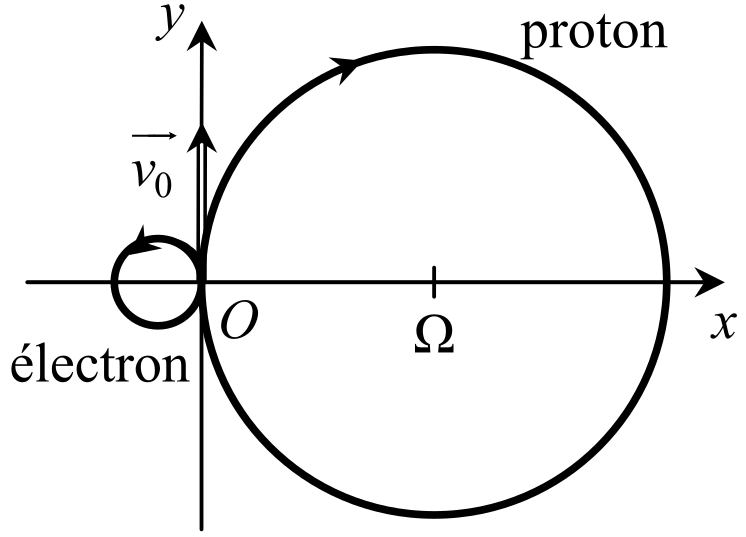
\includegraphics[width=0.4\linewidth]{chb_traj}
            % \captionsetup{justification=centering}
            \caption{Trajectoires pour un proton et un électron. \smallbreak
            Pour un proton,
            $\frac{v_0}{\w} = \frac{mv_0}{qB} >0$, donc la trajectoire est à
            droite, et le mouvement se fait dans le sens horaire. \smallbreak
            À l'inverse, pour
            l'électron la trajectoire est à gauche et se fait dans le sens direct, mais
            avec un rayon beaucoup plus petit puisque proportionnel à $m$.}
            \label{fig:chb_traj}
        \end{SCfigure}
    \item On réemploie le PFD~:
        \begin{gather*}
            m\af = q\vf\wedge\Bf -\lb\vf
            \Lra
            \left\{
                \begin{aligned}
                    m\xpp &= +qB\yp -\lb\xp \\
                    m\ypp &= -qB\xp -\lb \yp\\
                    m\zpp &= -\lb\zp
                \end{aligned}
            \right.
        \end{gather*}
        soit
        \begin{empheq}[box=\fbox, left=\empheqlbrace]{align}
            \label{eq:chb4}
            \xpp &= +\w\yp -\a\xp\\
            \label{eq:chb5}
            \ypp &= -\w\xp -\a\yp\\
            \label{eq:chb6}
            \zpp &= -\a\zp
        \end{empheq}
        Le mouvement reste plan, puisque la solution de l'équation~\ref{eq:chb6}
        est $\zp(t) = D\exp(-\a t)$, mais que $\zp(0) = 0 \Ra D = 0$, soit
        \fbox{$z = \cte =0$}.
    \item En posant, comme suggéré, $\uu = x + \jj y$, on combine
        $\eqref{eq:chb4}+\jj\eqref{eq:chb5}$ pour avoir
        \[\ddot{\uu} + (\a + \jw)\dot{\uu} = 0\]
        qui est une \textbf{équation différentielle d'ordre 2 sans ordre 0},
        donc d'ordre 1 en $\dot{\uu}$~: on trouve donc les solutions avec une
        simple exponentielle~:
        \begin{gather*}
            \dot{\uu}(t) = A\exp(-(\a + \jw)t)
            \\
            \qavec
            \dot{\uu}(0) = 0 + \jj v_0 = A
            \qsoit
            \dot{\uu}(t) = \jj v_0\exp(-(\a+\jw)t)\\
            \text{ainsi}\quad
            \uu(t) = \frac{\jj v_0}{-(\a+\jw)}\exp(-(\a+\jw)t) + B
            \qor
            \uu(0) = 0 \Lra B = \frac{\jj v_0}{\a+\jw}\\
            \text{finalement}\quad
            \boxed{\uu(t) = \frac{\jj
                v_0}{\a+\jw}\left(1-\exp(-(\a+\jw)t)\right)}
        \end{gather*}
        En mettant la fraction avec un dénominateur réel et en séparant les
        exponentielles~:
        \[
            \boxed{\uu(t) = \frac{\jj v_0\a + v_0\w}{\a^2+\w^2}
                \left(1-\exp(-\at)\exp(-\jwt)\right)}
            \]
        puis en prenant la partie
        réelle pour obtenir $x(t)$ et la partie imaginaire pour obtenir $y(t)$
        (\textbf{attention à bien distribuer la fraction}),
        \begin{empheq}[box=\fbox, left=\empheqlbrace]{align*}
            x(t) &= \frac{v_0\w}{\a^+\w^2}\left(1-\exp(-\at)\cos(\wt)\right)
                - \frac{v_0\a}{\a^2+\w^2}\exp(-\a t)\sin(\wt)\\
            y(t) &= \frac{v_0\w}{\a^+\w^2}\exp(-\a t)\sin(\wt)
                + \frac{v_0\a}{\a^2+\w^2}\left(1-\exp(-\at)\cos(\wt)\right)\\
        \end{empheq}
    \item Pour $t\ra\infty$, le point d'asymptote est
        \[
            \boxed{
                {\rm P}_{\infty} = \mqty(\DS\frac{v_0\w}{\a^2+\w^2}\\[1em]
                \DS\frac{v_0\a}{\a^2+\w^2}\\[1em]
                0)
            }
        \]
        \begin{minipage}{0.65\linewidth}
            La particule tourne toujours à cause des facteurs sinusoïdaux, mais le
            rayon de courbure diminue exponentiellement~: la trajectoire est une
            spirale, tournant toujours vers la droite pour un proton, et s'enroulant
            autour du point P$_{\infty}$.
        \end{minipage}
        \hfill
        \begin{minipage}{0.30\linewidth}
            %~\vspace{-12pt}
            \begin{center}
                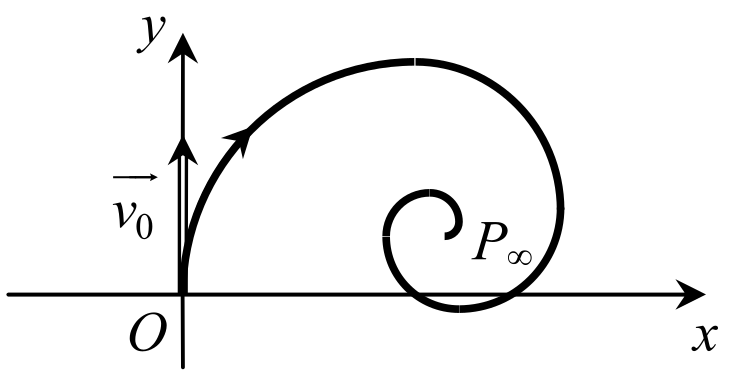
\includegraphics[width=\linewidth]{chb_spi}
            \end{center}
        \end{minipage}
\end{enumerate}

\end{document}
